\chapter{Evaluation}\label{sec:evaluation}


\begin{blockquote}
    \paragraph{Intent:} Performance evaluation 
    Structure:
    \begin{description}

        \item[Experimental setup] Optimization problems types, evaluation assumption and budget, repetition

        \item[Benhmark 1] Default Tutor-model(portfolio, thresholds) on plethora types of multiobjective problems
        \begin{enumerate}
            \item default Tutor-model parameters
            \item surrogate portfolio items
            \item Baseline: MOEA
        \end{enumerate}

        \item[Benhmark 2] Parameter selection of Tutor-model with the dynamic sampling plan
        \begin{enumerate}
            \item Parameters: prediction count, train/test split, stacking solutions. thresholds(x2), solver
            \item Subset of problems
            \item Baseline: Static vs Dynamic. Parameters tune
        \end{enumerate} 

        \item[Benhmark 3] Many-objective optimization. Objectives>10
        \begin{enumerate}
            \item Static Heterogeneous compositional surrogate vs. Homogeneous compositional surrogate
            \item Base line: MOEA or Random
        \end{enumerate}

        \item[Discussion] Results interpretation
    \end{description}
\end{blockquote}


In this section, we present the results obtained for proposed methods on test problems with diverse objective landscape and with a various number of search variables.

% ? MOEA is called globally convergent if the produced, non-dominated population converges to the true Pareto front while the number of generations goes to infinity.

For this study, we did not do extensive parameter tuning: NSGA-II and surrogates were run using their default settings.
\cite{kouwe2018benchmarking}

% --------------------------------------------------------------------------------------------
% ------------------------------------------------     Experimental setup     
% --------------------------------------------------------------------------------------------
\section{Experimental setup}
The measurements were performed on an Intel Core i7-8700CPU machine with 64G of memory using Fedora Server 29.

    % ---------------------------------     Optimization problems
    \subsection{Optimization problems}
    For comparison was selected several widespread synthetic benchmark suites. All of them are scalable in parameters space and some in objective space also. They simulate real life problem and have main related challenges such as multi-modality, different surface type, not uniform search space. All problems assumed global minimization for all objectives.

    The following property \cite{WFGref} could characterize optimization problems:
    \begin{itemize}
        \item Modality is the property of objectives surface. Test problems are either unimodal with one global optimum or multimodal with several local optima. Multimodal problems are more complicated than unimodal problems and more similar to real-world issues.
        \item The geometry of a Pareto optimal surface can directly influence the performance of the algorithm. Problems could be related to inner metrics of algorithms to estimate the dominance in population.
        \item The bias of landscape transformations impacts the search process by biasing the fitness landscape. This property means that uniformly distributed parameters mapping to predisposition area in objective space. This type of problem could be mode difficult if bias region is far away from the Pareto-optimal front.
        \item Many-to-one fitness mapping means that different parameter vector could produce the same objective vector. This property made the search more difficult to optimizers because increase likelihood of that parameters variations do not generate new objective vector.
    \end{itemize}

    % ! [===    Many-to-one, bias, Modality, geometry  ===]
        % -----------------------------  ZDT      
        \paragraph{ZDT} widespread test suite\cite{ZitzlerDT00} was conceived for two-objective problems and takes its name from its authors Zitzler, Deb and Thiele. Each test function involves a particular feature that is known to cause difficulty in the evolutionary optimization process, mainly in converging to the Pareto-optimal front.
        For benchmarks selected following problems:
        \begin{itemize}
            \item ZDT4: function has 21 local Pareto-optimal fronts and therefore is highly multi-modal. Also called multifrontal problems.
            \item ZDT6: function has a non-uniform search space: the Pareto-optimal solutions are non-uniformly distributed along the global Pareto front, and also the density of the solutions is lowest near the Pareto optimal front and highest away from the front
        \end{itemize}

        In their paper the authors propose a set of 6 different scalable problems all originating from a well thought combination of functions allowing, by construction, to measure the distance of any point to the Pareto front

        % -----------------------------   DTLZ
        \paragraph{DTLZ} benchmark suite\cite{DebTLZ05} was conceived for multiobjective problems with scalable fitness and objective dimensions and takes its name from its authors Deb, Thiele, Laumanns and Zitzler. All problems in this test suite are box-constrained continuous n-dimensional multi-objective problems, scalable in fitness dimension. Incidentally, there being multiple global optima is why many of the DTLZ problems are Pareto many-to-one. For benchmark evaluation, selected problem number 4 that has a dense area of solutions.

        % ------------------------------    WFG
        \paragraph{WFG} test suite \cite{WFGref} was designed to outperform the functionalities of previously implemented test suites. Important improvements and important challenges have been achieved in major type of problems. Also, problems with dependencies between position and distance-related parameters are included. The WFG test suite was introduced by Simon Huband, Luigi Barone, Lyndon While, and Phil Hingston. The following problems are selected for benchmarking:
            \begin{itemize}
                \item WFG1: This problems skews the relative significance of different parameters by employing different weights in the weighted sum reduction. Also, this problem is unimodal and with a convex and mixed Pareto optimal geometry
                \item WFG4: This is a multimodal problem with a concave Pareto optimal geometry. The multimodality of this problem has large "hills" that make it more complicated for optimization. 
            \end{itemize}


        % ==== multi-objective test problems
        \begin{table}[]
            \caption{Selected multi-objective test problems\label{bench_problems}}
            \centering
            \resizebox{\textwidth}{!}{%
                \begin{tabular}{@{}cccccc@{}}
                \toprule
                \multirow{2}{*}{\textbf{Problem}} &
                \multirow{2}{*}{\textbf{Objective}} &
                \multirow{2}{*}{\textbf{Modality}} &
                \multirow{2}{*}{\textbf{Geometry}} &
                \multicolumn{2}{c}{\textbf{Landscape}} \\ \cmidrule(l){5-6}
                            &                 &                      &               & \textbf{Bias}    & \textbf{\begin{tabular}[c]{@{}c@{}}Many-to-one \\ mappings\end{tabular}} \\ \midrule
                \textbf{ZDT4}  & bi-objective    & unimodal, multimodal & convex        & -                & -                                                                        \\
                \textbf{ZDT6}  & bi-objective    & multimodal           & concave       & +                & +                                                                        \\
                \textbf{DTLZ4} & multi-objective & unimodal             & concave       & +                & +                                                                        \\
                \textbf{WFG1}  & multi-objective & unimodal             & convex, mixed & polynomial, flat & +                                                                        \\
                \textbf{WFG4}  & multi-objective & multimodal           & concave       & -                & +                                                                       \\ \bottomrule
                \end{tabular}%
            }
        \end{table}



    % ---------------------------------     Optimization search
    \subsection{Optimization search}
    In benchmarks, all genetic algorithms operate with population size equal to 100. Other parameters do not change. 
    Default solvers for surrogates selected as genetic control with MOEA/D and NSGA2. Intuition of why this is a right combination: NSGA2 gave stable results with a proper distribution of points in Pareto-front approximation; MOEA/D have good exploration quality with low generation count.

    %! [ ====   NSGA2 vs MOEA/D  ====]

    % ---------------------------------    Portfolio
    \subsection{Surrogate portfolio}
        For a default surrogate portfolio were selected a most popular and perspective models. All of them have advantages and drawbacks concerning the concrete problem, although some surrogate models are indeed more universal but require much more time and prior information. From multi-objective models, there is Gaussian Process Regressor that commonly used for model-based optimization. For this type of model should be specified by the prior's covariance. It is defined by passing a kernel object, the hyperparameters of which are optimized during extrapolations of the samples. The kernel for this benchmark is selected from a Rasmusen and illustrate an intricate design. The Gaussian Process Regressor with this kernel is used to extrapolate the $CO_2$ concentration as a function of the time $t$. The kernel consists of several components that calibrate to represent a long term, periodic and medium components. Even though this kernel is from another domain, it does give good extrapolation quality for the regression model. Unfortunately, the build time is significant and grows with samples size and dimensionality.

        From compositional models were selected three single-objective models that give $3^{obj}$ possible surrogate hypothesis combinations. 
        \begin{itemize}
            \item SVR model with RBF kernel. SVR, in general, uses the same principles as the SVM for classification with the main idea is to minimize error, individualizing the hyperplane which maximizes the margin. With a motivation to extend the SVR to non-linear data, the kernel function transforms the data into a higher dimensional feature space that could be linearly separate.
            \item Multi-layer Perceptron regressor (MLPRegressor) with three hidel layers. A neural network is a popular and influential approach to the fitness landscape.
            \item Gradient Boosting Regressor that uses an ensemble decision tree regressors to produce a single model. Building process goes iteratively, at each step, a new tree is trained against the negative gradient of the loss function, that improve results in the previous step. This method accurate and efficient that can be used in a variety of areas
        \end{itemize}
        
        As a result, for bi-objective problems, there are no more than ten possible surrogate hypothesis, including multi-objective Gaussian Process Regressor. All training and validation models perform in parallel. For a benchmark purpose, at each optimization round surrogate portfolio stay the same. 

    % ---------------------------------    Benchmark baseline
    \subsection{Benchmark baseline}
    The developed approach in this thesis(class TutorModel) was compared with Hypermapper\cite{nardi2019practical}, that focus on multi-objective parameter tuning with various types of parameters. Hypermapper used several randomized decision forests models, one for each objective, and appply Bayesian optimization to find optimal points. General idea ground in scaling several surrogates to single-objective criteria and optimize it with Bayesian optimization. Hypermapper was succesfuly used in autotuning computer vision aplications. Hypermapper does not specify an initial sampling size. That is why we select it as default population size for MOEA (100 points).

    NSGA2 was selected as the baseline for optimization. It is suggested that the algorithms in benchmark should be approximated in quality to the best result(NSGA2 10k evaluations) but at the same time, be better than the basic approach with a limited budget(NSGA2 1k evaluations).

% --------------------------------------------------------------------------------------------
% ---------------------       Benchmark 1: Model-tutor: Portfolio with compositional surrogates 
% --------------------------------------------------------------------------------------------
\section{Benchmark 1: Portfolio with compositional surrogates. Dynamic sampling plan. [RQ1, RQ2]}
    Results showed that the sampling plan dynamically collects a different amount of samples based on a current problem (Figure \ref{fig:changing_models}). When samples are enough, several models could periodically swap as best available. Furthermore, with growing samples set, models give more stable results, and changes become less frequent. In the case of WFG1 problem(\ref{fig:wfg1_models_60}) best accuracy for non-dominated point gave the compositional model with GPR for each objective. In WFG problem, the same compositional model goes ahead other models in the portfolio, but after samples size increased, multi-objective GP regression was on the top.

    % === TutorM: surrogate portfolio in action
    \begin{figure}
        \centering
        \begin{subfigure}{\textwidth}
            \includegraphics[width=\textwidth]{content/images/dtlz4_models}
            \caption{DTLZ4: Sampling plan bis 210 examples}
            \label{fig:dtlz4_models_210}
        \end{subfigure}
        % \hfill
        
        \begin{subfigure}{\textwidth}
            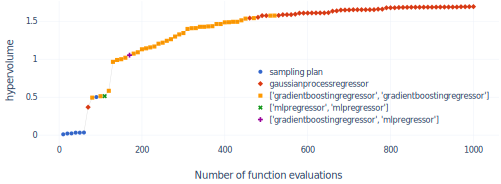
\includegraphics[width=\textwidth]{content/images/wfg1_models}
            \caption{WFG1: Sampling plan bis 60 examples}
            \label{fig:wfg1_models_60}
        \end{subfigure} 

        \caption[The optimization process with dinamic sampling plan and surrogate portfolio.]{The optimization process with dinamic sampling plan and surrogate portfolio. Plots are shown in which step sampling plan was used or which model gives the best accuracy on the test set. More hypervolume is better.}
        \label{fig:changing_models}    
    \end{figure}


    Figure \ref{fig:changing_models} illustrates how improves the solutions for ZDT6 problem. Initially, it could be notest that TutorM considerably outperforms NSGA2 and Hypermapper right from the start of their optimisation process (Fig \ref{fig:zdt6_dist}). TutorM after 300 evaluations, corresponds to the stable near-optimal solution. Besides to interpreter results more involved, non-dominated size should be analysed. ZDT6 landscape has flat regions with local Pareto-front. Hypermapper gets stuck in some of them as evidenced by the serrated graph (Fig \ref{fig:zdt6_ndf}). The drop occurs when discovering a new point in the other Pareto-optimal front. NSGA2 stagnate and comparable to random search due to the many-to-one fitness mapping. Solutions from the population do not have enough sparsity in objective space to detect optimal search direction. TutorM detects global Pareto front straightway and increases Pareto-optimal solutions slowly that alike to solutions from nsga2 with 10k evaluations (Fig \ref{fig:zdt6_front}).

    % === ZDT6
    \begin{figure}
        \centering
        \begin{subfigure}{\textwidth}
            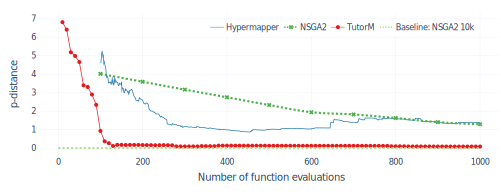
\includegraphics[width=\textwidth]{content/images/zdt6_dist}
            \caption{ZDT6: p-distance to real Pareto-front}
            \label{fig:zdt6_dist}
        \end{subfigure} 
        % \hfill
        
        \begin{subfigure}{\textwidth}
            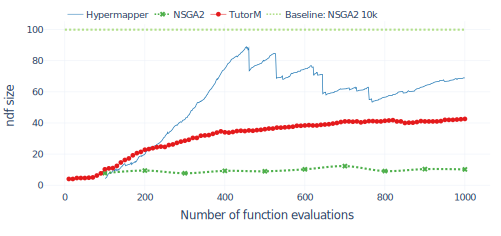
\includegraphics[width=\textwidth]{content/images/zdt6_ndf}
            \caption{ZDT6: Size of a non-dominated subset of an evaluated examples}
            \label{fig:zdt6_ndf}
        \end{subfigure} 

        \begin{subfigure}{\textwidth}
            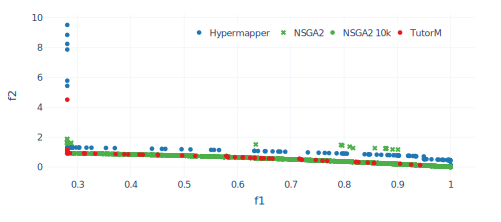
\includegraphics[width=\textwidth]{content/images/zdt6_front}
            \caption{ZDT6: Pareto-front approximation after 1000 function evaluations}
            \label{fig:zdt6_front}
        \end{subfigure} 

        \caption[Comparison of solutions on ZDT6 problem]{A complex comparison of solutions on ZDT6 problem. Final non-dominated points are used to estimate Pareto-optimal solutions.}
        \label{fig:changing_models}    
    \end{figure}


    As shown in Figure \ref{fig:wfg_14}, TutorM could also outperform the MOEA baseline in 10k evaluations(\ref{sub@fig:wfg1_front}). WFG1 has flat landscape regions hence the convergence of genetic algorithms significantly deteriorates. Hypermapper increase count of non-dominated points, regardless it is local optimum and most samples stack in a small region. Nsga2 after 1000 function evaluations also have high-density regions which could be improved with spending more effort to evaluations. The TutorM has several dozen of Pareto-optimal points from all over the budget, that significantly outperforms Hypermapper and nsga2 even with 10k evaluations. 
    From WFG4 use case, all over all approaches gain near-optimal results(\ref{fig:wfg4_front}), but significant advantage over TutorM as it provides an extensive set of points(\ref{fig:wfg4_ndf}) that are well distributed at the Pareto front.


    % === WFG1 and WFG4
    \begin{figure}
        \centering
        \begin{subfigure}{\textwidth}
            \begin{subfigure}{0.5\textwidth}
                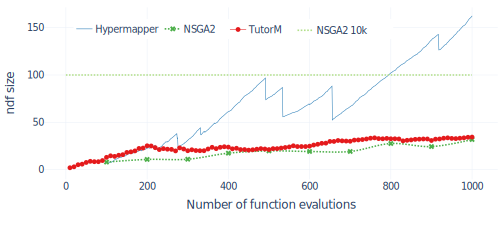
\includegraphics[width=\textwidth]{content/images/wfg1_ndf}
                \caption{WFG1: Size of a non-dominated subset of an evaluated examples}
                \label{fig:wfg1_ndf}
            \end{subfigure} 
            \begin{subfigure}{0.5\textwidth}
                \includegraphics[width=\textwidth]{content/images/wfg1_front}
                \caption{WFG1: Pareto-front approximation}
                \label{fig:wfg1_front}
            \end{subfigure} 
        \end{subfigure} 

        
        % ?\hfill


        \begin{subfigure}{\textwidth}
            \begin{subfigure}{0.5\textwidth}
                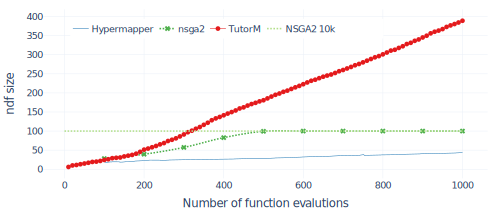
\includegraphics[width=\textwidth]{content/images/wfg4_ndf}
                \caption{WFG4: Size of a non-dominated subset of an evaluated examples}
                \label{fig:wfg4_ndf}
            \end{subfigure} 
            \begin{subfigure}{0.5\textwidth}
                \includegraphics[width=\textwidth]{content/images/wfg4_front}
                \caption{WFG4: Pareto-front approximation}
                \label{fig:wfg4_front}
            \end{subfigure}
        \end{subfigure} 
        
 

        \caption[Comparison of solutions on ZDT6 problem]{A complex comparison of solutions on ZDT6 problem. Final non-dominated points are used to estimate Pareto-optimal solutions.}
        \label{fig:wfg_14}    
    \end{figure}





    \begin{table}[]
        \centering
        \resizebox{\textwidth}{!}{%
        \begin{tabular}{@{}ccccccc@{}}
        \toprule
                                             & \textbf{Metric}        & \textbf{ZDT4} & \textbf{ZDT6} & \textbf{DTLZ4} & \textbf{WFG1} & \textbf{WFG4} \\ \midrule
        \multirow{4}{*}{\textbf{TutorM}}     & \textbf{hypervolume}   & 99,45\%       & 99,01\%       & 99,27\%        & 115,60\%      & 95,95\%       \\
                                             & \textbf{p-distance}    & 1,336         & 0,522         & 0,022          & -             & -             \\
                                             & \textbf{ndf-size}      & 183,022       & 31,528        & 119,308        & 24,158        & 183,244       \\
                                             & \textbf{space-metrics} & 0,103         & 0,142         & 0,186          & 0,129         & 0,032         \\ \midrule
        \multirow{4}{*}{\textbf{NSGA2}}      & \textbf{hypervolume}   & 97,57\%       & 87,46\%       & 95,87\%        & 45,01\%       & 91,87\%       \\
                                             & \textbf{p-distance}    & 1,391         & 1,872         & 0,022          & -             & -             \\
                                             & \textbf{ndf-size}      & 44,000        & 11,455        & 39,900         & 20,164        & 82,436        \\
                                             & \textbf{space-metrics} & 0,176         & 0,355         & 0,268          & 0,228         & 0,038         \\ \midrule
        \multirow{4}{*}{\textbf{Hypermaper}} & \textbf{hypervolume}   & 96,82\%       & 66,95\%       & 81,29\%        & 40,66\%       & 74,09\%       \\
                                             & \textbf{p-distance}    & 2,024         & 1,850         & 0,076          & -             & -             \\
                                             & \textbf{ndf-size}      & 28,908        & 52,746        & 10,743         & 81,512        & 30,158        \\
                                             & \textbf{space-metrics} & 0,1386        & 0,11621       & 0,5282         & 0,0870        & 0,1032        \\ \midrule
        \multirow{4}{*}{\textbf{\begin{tabular}[c]{@{}c@{}}NSGA2\\ 10k eval\end{tabular}}} & \textbf{hypervolume}      & 100,00\% & 100,00\% & 100,00\% & 100,00\% & 100,00\% \\
                                             & \textbf{p-distance}    & 0,152         & 0,256         & 0,002          & -             & -             \\
                                             & \textbf{ndf-size}      & 93,901        & 79,776        & 93,990         & 85,196        & 98,087        \\
                                             & \textbf{space-metrics} & 0,033         & 0,074         & 0,039          & 0,051         & 0,016         \\ \bottomrule
        \end{tabular}%
        }
        \end{table}


% --------------------------------------------------------------------------------------------
% ---------------------       Benchmark 2: Dynamic sampling plan and parameter selection
% --------------------------------------------------------------------------------------------
\section{Benchmark 2: Inner parameters}

    \subsection{Model-tutor parameters}
    \begin{itemize}
        \item \texttt{PredictTutor} class
            \begin{itemize}
                \item Surrogate portfolio
                \item Cross-Validation rounds
                \item Cross-Validation threshold
                \item Train/test split
                \item Test threshold
            \end{itemize}
        \item Optimization search algorithm
        \item Pareto front infill-criteria (Non-dominated score/Solutions combination)
        \item Prediction count
    \end{itemize}

    %! [ Hypermapper baseline; ModelTutor and change quality (grid plot)] iterations

    %! [ Hypermapper baseline; ModelTutor and change quality (bubble chart) ] Deviations



% --------------------------------------------------------------------------------------------
% ---------------------       Benchmark 3: Many-objective optimization, scaling
% --------------------------------------------------------------------------------------------
\section{Benchmark 3: Many-objective optimization. Scaling. RQ1.1}
    For evaluation scalability property for the compositional model, problem XXX was selected.

    Objectives: 1) detect iterative improvement, a convergence of the primary metric 2) time for evaluation

    Usecases: GausianModel, GausianModel + Gradient, GausianModel + random forest, 

    Scale: objectives - 2,4,8,10; params - 2,4,8,10

    % ! [ Hypermapper baseline; X - objectives Y - p-distance/time]



% --------------------------------------------------------------------------------------------
% ---------------------       Benchmark 4: real world scenario
% --------------------------------------------------------------------------------------------
\section{Benchmark 4: Parameter tuning of SVM}

    % ! [ Hypermapper baseline; SVM score in iterations]


% --------------------------------------------------------------------------------------------
% ------------------------------------------------     Discussion 
% --------------------------------------------------------------------------------------------
\section{Discussion}

Up to now, most papers used the
The quality of the results obtained with X was similar to the results obtained with Y, but with significantly fewer exactly evaluated solutions during the optimization process. 


consume an inordinate amount of time.

% \paragraph{Neuroevolution of augmenting topologies}
%  *Training Neural Networks (especially deep ones) is hard and has many issues (non-convex cost functions - local minima, vanishing and exploding gradients etc.).

%  Training Neural Networks (NNs) with Genetic Algorithms (GAs) is not only feasible, there are some niche areas where the performance is good enough to be used frequently. A good example of this is Neuroevolution of augmenting topologies or NEAT, which a successful approach to generating controllers in simple environments, such as games.

%  In the more general case though, the approach does not scale well to large, deep networks with many parameters to tune.

%  Genetic algorithms and other global searches for optimal parameters are robust in ways that gradient-based algorithms are not. For instance, you could train a NN with step function activations, or any other non-differentiable activation functions. They have weaknesses elsewhere. One thing relevant in the case of GAs used for NNs, is that weight parameters are interchangeable in some combinations but heavily co-dependent in other combinations. Merging two equally good neural networks with different parameters - which you would do in cross-over in a GA - will usually result in a third network with poor performance. NEAT's success is partially in finding a way to address that issue by "growing" the NN's connections and matching them up between similar neural networks.

%  Gradient-based approaches are much more efficient. In general, and not just in domain of NNs, if you can calculate gradient of a function with respect to parameters, then you can find optimal parameters faster than most other optimising techniques. An accurate gradient guarantees at least a small improvement from a single evaluation, and most other optimisers fall into a generate-and-retry paradigm which cannot make that kind of guarantee. The weakness of tending to find local optima has turned out not be a major hindrance for the loss functions in NNs, and has been tackled with some degree of success using extensions to basic gradient descent such as momentum, RPROP, Adam etc.

%  In practice on a large multi-layer network, gradient methods are likely orders of magnitude faster than GA searches such as NEAT for finding network parameters. You won't find any GA-trained CNNs that solve ImageNet, or even MNIST, where the GA has found the network weights unaided. However, GAs, or at least some variants of them, are not 100'\%' ruled out. For instance this 2017 blog reviews recent papers including Large-Scale Evolution of Image Classifiers which explores using GAs to discover NN hyperparameters which is an important task in machine learning, and not very tractable using gradient-based methods.
% Test problems  
% Experimental setup
% Results
% Discussion



% non-separable
% or have a deceptive fitness landscape



% On the left side the learning curve of a naive Bayes classifier is shown for the digits dataset. Note that the training score and the cross-validation score are both not very good at the end. However, the shape of the curve can be found in more complex datasets very often: the training score is very high at the beginning and decreases and the cross-validation score is very low at the beginning and increases. On the right side we see the learning curve of an SVM with RBF kernel. We can see clearly that the training score is still around the maximum and the validation score could be increased with more training samples.
% https://scikit-learn.org/0.15/auto_examples/plot_learning_curve.html